\documentclass{beamer}
\usepackage{beamerthemesplit}
\usepackage{wrapfig}
\usetheme{SPbGU}
\usepackage{pdfpages}
\usepackage{amsmath}
\usepackage{mathtools}
\usepackage{cmap} 
\usepackage[T2A]{fontenc} 
\usepackage[utf8]{inputenc}
\usepackage[english,russian]{babel}
\usepackage{indentfirst}
\usepackage{amsmath}
\usepackage{tikz}
\usepackage{multirow}
\usepackage{multicol}
\usepackage{array}
\usepackage[noend]{algpseudocode}
\usepackage{algorithm}
\usepackage{algorithmicx}
\usepackage{minted}
\usepackage{verbatim}
\usepackage[linguistics]{forest}
\usetikzlibrary{shapes,arrows}
\usepackage{fancyvrb}
\newtheorem{rutheorem}{Теорема}
\newtheorem{ruproof}{Доказательство}
\newtheorem{rudefinition}{Определение}
\newtheorem{rulemma}{Лемма}
\beamertemplatenavigationsymbolsempty
\setbeamertemplate{itemize item}[circle]
\setbeamertemplate{enumerate item}[circle]
\newcommand{\derives}[1][*]{\xRightarrow[]{#1}}


\title[]{Теория автоматов и формальных языков}
\subtitle[]{Введение}
\institute[]{
Санкт-Петербургский государственный электротехнический университет <<ЛЭТИ>>\\
}

\author[]{Екатерина Вербицкая}

\date{5 сентября 2019}

\definecolor{orange}{RGB}{179,36,31}

\begin{document}
{
  \begin{frame}
    \titlepage
  \end{frame}
}

\begin{frame}[fragile]
  \transwipe[direction=90]
  \frametitle{О чем этот курс?}
  Теория автоматов и формальных языков изучает:
  \begin{itemize}
    \item Математические модели для описания языков
    \item Абстрактные машины для работы с языками
  \end{itemize}
  
  Также рассматриваются:
  \begin{itemize}
    \item Подходы к описанию синтаксиса языков
    \item Подходы к описанию ``смысла'' программ и предложений
    \item Принципиальные ограничения механизмов для работы с языками
  \end{itemize}
\end{frame}

\begin{frame}[fragile]
  \transwipe[direction=90]
  \frametitle{Какие бывают языки?}
  \pause
  \begin{itemize}
    \item Естественные 
    \begin{itemize}
      \item Русский, английский...
    \end{itemize}    
    \pause
    \item Искусственные
    \begin{itemize}
      \item Эсперанто, ложбан...
      \item Клингонский, эльфийский...
      \pause
      \item C++, Python, Java, C\#, Haskell, OCaml, Perl, Coq, Agda...
    \end{itemize}
  \end{itemize}
\end{frame}

\begin{frame}[fragile]
  \transwipe[direction=90]
  \frametitle{Где можно встретить языки?}
  В повседневной жизни: 
  \begin{itemize} 
    \item при разговоре, в переписке
    \item на заборах, на стенах гробниц
    \item в собственной голове при формулировке мыслей... 
  \end{itemize} 
\pause ~\\  
  При работе с различными \textbf{языковыми процессорами}:
  \begin{itemize}
    \item текстовыми редакторами
    \item компиляторами, интерпретаторами, трансляторами
    \item средами разработки...
  \end{itemize}
\pause ~\\
  Все нуждаются в \textbf{формализованном представлении} языка
\end{frame}

\begin{frame}[fragile]
  \transwipe[direction=90]
  \frametitle{Два аспекта спецификации языка программирования}
  \begin{itemize}
    \item Синтаксис --- правила построения программ из символов
    \begin{itemize}
      \item Форма
    \end{itemize}
    \item Семантика --- правила истолкования программ
    \begin{itemize}
      \item Смысл
    \end{itemize}
  \end{itemize}
\end{frame}

\begin{frame}[fragile]
  \transwipe[direction=90]
  \frametitle{Пример: английский язык}

\begin{center}
    You know nothing, Jon Snow
\end{center}
  
  \begin{itemize}
    \item Синтаксис
    \begin{itemize}
      \item \dots
      \item Порядок слов в предложении: подлежащее, дополнение сказуемое, все остальное
      \item Обращение обособляется запятыми
      \item \dots
    \end{itemize}
    \item Семантика
    \begin{itemize}
      \item Говорящий обращается к Джону Сноу, утверждая, что Джон ничего не знает
    \end{itemize}
  \end{itemize}
\end{frame}

\begin{frame}[fragile]
  \transwipe[direction=90]
  \frametitle{Пример: язык арифметических выражений}
 
 \begin{center}
    $1 * (2 + 3) / 4 - 5$ 
 \end{center}
  
  \begin{itemize}
    \item Синтаксис
    \begin{itemize}
      \item \textbf{Терм}: последовательность цифр или любое \textbf{выражение} в скобках
      \item \textbf{Слагаемое}: последовательность \textbf{термов}, соединненых знаками умножения и деления
      \item \textbf{Выражение}: последовательность \textbf{слагаемых}, соединенных знаками сложения и вычитания (перед первым \textbf{слагаемым} может стоять минус)
    \end{itemize}
    \item Семантика
    \begin{itemize}
      \item Значение арифметического выражения
      \pause
      \begin{itemize}
        \item $-3.75$
        \item $-4$
      \end{itemize}
    \end{itemize}
  \end{itemize}
\end{frame}


\begin{frame}[fragile]
  \transwipe[direction=90]
  \frametitle{Пример: синтаксис if-выражений}
\begin{columns}
  \begin{column}{0.5\textwidth}
    \begin{minted}[frame=single]{python}
if temperature > 23:
  print('Wear shorts.')
else:
  print('Wear long pants.')
    \end{minted}
  \end{column}

  \begin{column}{0.5\textwidth}
    \begin{minted}[frame=single]{c}
if ( temperature > 23 ) {      
  cout<<"Wear shorts.\n";
}
else 
  cout<<"Wear long pants.\n"; 
}
    \end{minted}
  \end{column}
\end{columns}

\vspace{30pt}

\begin{columns}
  \begin{column}{0.5\textwidth}
    \begin{minted}[frame=single]{haskell}
if temperature > 23 
then print "Wear shorts."
else print "Wear long pants."
    \end{minted}
  \end{column}

  \begin{column}{0.5\textwidth}
    \begin{minted}[frame=single]{scheme}
(if (> temperature 23) 
  (print "Wear shorts.")
  (print "Wear long pants."))  
    \end{minted}
  \end{column}
\end{columns}

\end{frame}

\begin{frame}[fragile]
  \transwipe[direction=90]
  \frametitle{Что такое язык?}
  \pause
  
  \begin{center}
    \textbf{Язык} --- множество строк
  \end{center}
\end{frame}

\begin{frame}[fragile]
  \transwipe[direction=90]
  \frametitle{Что такое множество?}
  \pause

\begin{center}
    \textbf{Множество} --- набор уникальных элементов
\end{center}

  \pause 
  \begin{itemize}
    \item $x \in X$: $x$ --- элемент множества $X$ ($x$ принадлежит $X$)
    \item $x \notin X$: $x$ не является элементом множества $X$ \\ ($x$ не принадлежит $X$)
    \item Уникальность, неупорядоченность: $\{ 13, 42 \} = \{ 42, 13 \} = \{ 42, 13, 42 \}$
    \item Универсальное множество (универсум $\mathcal{U}$): множество всех мыслимых объектов
    \begin{itemize}
      \item $\mathbb{N} = \{ 1, 2, 3, \dots \}$
      \item $\mathbb{Z} = \{ \dots, -2, -1, 0, 1, 2, \dots \}$
      \item $\mathbb{Q} = \{ m / n \mid m, n \in \mathbb{Z}; n \neq 0 \}$
    \end{itemize}
  \end{itemize}
\end{frame}

\begin{frame}[fragile]
  \transwipe[direction=90]
  \frametitle{Подмножества}
  $A$ является \textbf{подмножеством} $B$ тогда и только тогда, когда все элементы $A$ являются элементами $B$
  
  \begin{center}
     $ A \subseteq B \iff \forall x : x \in A \Rightarrow x \in B $   
  \end{center} 
  
  \pause 
  \begin{itemize}
    \item $\{ 13, 42 \} \subseteq \{ 7, 13, 37, 42, 99 \}$
    \item $\{ 1, 3, 5, ...\} \subseteq \mathbb{N} $
    \item $\mathbb{N} \subseteq \mathbb{Z}$
    \item $\forall A : A \subseteq A$
  \end{itemize}
  \begin{itemize}
    \item Пустое множество ($\varnothing$): множество без элементов
    \begin{itemize}
      \item $\forall x : x \notin \varnothing$
      \item $\forall A : \varnothing \subseteq A$
    \end{itemize}
  \end{itemize}
\end{frame}

\begin{frame}[fragile]
  \transwipe[direction=90]
  \frametitle{Подмножества}
  Множества $A$ и $B$ \textbf{равны} тогда и только тогда, когда $A$ является подмножеством $B$ и $B$ является подмножеством $A$  
  
  \begin{center}
    $ A = B \iff A \subseteq B $ и $ B \subseteq A$
  \end{center}
  \pause
  $A$ является \textbf{строгим подмножеством} $B$ тогда и только тогда, когда $A$ является подмножеством $B$, но они не равны друг другу
  
  \begin{center}
     $ A \subset B \iff A \subseteq B $ и $ A \neq B $   
  \end{center} 
  
  \pause 
  \begin{itemize}
     \item $\forall x : \varnothing \subset \{ x \}$
     \item $\mathbb{N} \subset \mathbb{Z}$
     \item $\mathbb{Z} \not\subset \mathbb{N}$
     \item $\forall A: A = A $ и $ A \not\subset A $

  \end{itemize}
\end{frame}

\begin{frame}[fragile]
  \transwipe[direction=90]
  \frametitle{Множество всех подмножеств (powerset)}
  \textbf{Множество всех подмножеств} множества $A$ состоит из всех подмножеств $A$
  
  \begin{center}
    $2^A = \{ B \mid B \subseteq A \}$
  \end{center}
  
  \begin{itemize}
    \item $\forall A: \varnothing \in 2^A$
    \item $\forall A: A \in 2^A$
    \item $A = \{ 0, 1 \} \Rightarrow \{ \varnothing, \{ 0 \}, \{ 1 \}, \{ 0, 1 \} \} $
  \end{itemize}
  
  \pause 
  Сколько элементов может быть в множестве всех подмножеств?
\end{frame}

\begin{frame}[fragile]
  \transwipe[direction=90]
  \frametitle{Операции над множествами}
\[  
  \begin{array}{rccl}
     \text{Объединение: } & A \cup B &=& \{ x \mid x \in A  \text{ или } x \in B \} \\[\medskipamount]
     \text{Пересечение: } & A \cap B &=& \{ x \mid x \in A \text{ и } x \in B \} \\[\medskipamount]
     \text{Разность: }    & A \setminus B &=& \{ x \mid x \in A \text{ и } x \notin B \} \\[\medskipamount]
     \text{Дополнение: } & \overline{A} &=& \{ x \mid x \in \mathcal{U} \text{ и } x \notin A \} = \mathcal{U} \setminus A 
  \end{array}
\]

\end{frame}

\begin{frame}[fragile]
  \transwipe[direction=90]
  \frametitle{Строки: неформально}
  \pause
  
  \begin{center}
    \textbf{Строка} --- последовательность символов
  \end{center}
\end{frame}

\begin{frame}[fragile]
  \transwipe[direction=90]
  \frametitle{Алфавит}
  \begin{itemize}
    \item \textbf{Алфавит} ($\Sigma$) --- конечное множество (атомарных, неделимых) \emph{символов}
    \begin{itemize}
      \item $\{ a, b, c, \dots, z \}$
      \item $\{ \alpha, \beta, \gamma, \dots, \omega \}$
      \item $\{ 0, 1 \}$
      \item $\{ \text{\underline{let}, \underline{in}, \underline{where}, \dots} \}$
    \end{itemize}    
  \end{itemize}
\end{frame}

\begin{frame}[fragile]
  \transwipe[direction=90]
  \frametitle{Цепочка}
  \begin{itemize}
    \item \textbf{Цепочка (предложение, слово, \emph{строка})} --- любая конечная 
последовательность символов алфавита
    \begin{itemize}
      \item cat
      \item $\kappa \alpha \tau$
      \item 011000110110000101110100
      \item \verb!main = putStrLn . show . inc 2 where inc = \x -> x + 1!
    \end{itemize}    
    \item \textbf{Пустая цепочка $\varepsilon$} --- цепочка, не содержащая ни одного символа
    \begin{itemize}
      \item $\varepsilon$ не является символом алфавита
    \end{itemize}   
  \end{itemize}
\end{frame}

\begin{frame}[fragile]
  \transwipe[direction=90]
  \frametitle{Конкатенация строк}
  \begin{itemize}
    \item \textbf{Конкатенация строк $\alpha$ и $\beta$ $(\alpha \cdot \beta = \alpha \beta)$} --- результат 
приписывания строки $\beta$ в конец строки $\alpha$
    \begin{itemize}
      \item $\forall \alpha \beta \gamma : (\alpha \cdot \beta) \cdot \gamma = \alpha \cdot (\beta \cdot \gamma)$
      \item $\forall \alpha : \alpha \cdot \varepsilon = \varepsilon \cdot \alpha = \alpha$
    \end{itemize}
  \end{itemize}
\end{frame}

\begin{frame}[fragile]
  \transwipe[direction=90]
  \frametitle{Пример: арифметические выражения}
  \begin{itemize}
    \item Алфавит $\Sigma = \{ 0, 1, 2, 3, 4, 5, 6, 7, 8, 9, +, -, *, /, (, ) \}$
    \item $1 * (2 + 3) / 4 - 5 =$ \\ $ 1 \cdot * (2 + 3) / 4 - 5 =$ \\ $ 1 * (2 + 3) \cdot / 4 - 5 = $\\ $ 1 \cdot * \cdot (\cdot 2 \cdot + \cdot 3 \cdot) \cdot / \cdot 4 \cdot - \cdot 5 = $ \\ $ 1 * (2 + 3) / 4 - 5 \cdot \varepsilon$
    \item Является ли $\varepsilon$ арифметическим выражением?
  \end{itemize}
\end{frame}


\begin{frame}[fragile]
  \transwipe[direction=90]
  \frametitle{Операции над строками}
  \begin{itemize}
    \item \textbf{Обращение (реверс) цепочки $a^R$} --- цепочка, символы которой записаны в обратном порядке
    \begin{itemize}
      \item Если $x = abc$, то $x^R = cba$
      \item $\varepsilon^R = \varepsilon$
    \end{itemize}
    \item \textbf{$n-$я степень цепочки $a^n$} --- конкатенация $n$ повторений цепочки
    \begin{itemize}
      \item $a^0 = \varepsilon$
      \item $a^n = a \cdot a^{n-1} = a^{n-1} \cdot a$
    \end{itemize}
    \item \textbf{Длина цепочки $|a|$} --- количество составляющих ее символов
    \begin{itemize}
      \item $|babb| = 4$
      \item $|babb|_a = 1, |babb|_b = 3, |babb|_c = 0$
      \item $|\varepsilon| = 0$
    \end{itemize}
  \end{itemize}
\end{frame}

\begin{frame}[fragile]
  \transwipe[direction=90]
  \frametitle{Формальный язык}
  \begin{itemize}
    \item $\Sigma$ --- алфавит
    \begin{itemize}
      \item $\Sigma = \{ 0, 1 \}$
    \end{itemize}
    \item $\Sigma^*$ --- множество, содержащее все цепочки в алфавите $\Sigma$, включая пустую цепочку
    \begin{itemize}
      \item $\Sigma^*=  \{ \varepsilon, 0, 1, 00, 11, 01, 10, 000, 001, 011, ... \}$
      \item Сколько может быть элементов в $\Sigma^*$?
      \pause
    \end{itemize}
    \item $\Sigma^+ = \Sigma^* \setminus \{ \varepsilon \} $ 
    \begin{itemize}
      \item $\Sigma^+ = \{0, 1, 00, 11, 01, 10, 000, 001, 011, \dots \}$
      \item Сколько может быть элементов в $\Sigma^+$?
      \pause
    \end{itemize}
  \end{itemize}
  \begin{itemize}
    \item \emph{Формальный язык} в алфавите $\Sigma$ --- подмножество множества всех цепочек в этом алфавите. 
    \begin{itemize} 
      \item Для любого языка $L$ (в алфавите $\Sigma$) справедливо $L \subseteq \Sigma^*$
      \item $L = \{ 0, 00, 000, \dots\} \subset \{0, 1\}^*$
      \item $L = \{ 0, 0101, 011011011, \dots\} \subset \{0, 1\}^*$
    \end{itemize}
  \end{itemize}
\end{frame}

\begin{frame}[fragile]
  \transwipe[direction=90]
  \frametitle{Метаязык}
  \begin{itemize}
    \item Язык, на котором дано описание языка
    \begin{itemize}
      \item Естественный язык
      \pause
      \item \textbf<5>{Язык металингвистических формул Бэкуса (БНФ)}
      \pause \item Синтаксические диаграммы
      \pause \item Грамматики 
      \item $\dots$
    \end{itemize}
  \end{itemize}
\end{frame}


\begin{frame}[fragile]
  \transwipe[direction=90]
  \frametitle{БНФ ---  Бэкуса-Наура форма}
  \begin{itemize}
    \item \textbf{Символ} --- элементарное понятие языка
    \begin{itemize}
      \item $+$ означает сложение в языке арифметических выражений
    \end{itemize}
    \item \textbf{Метапеременная} --- сложное понятие языка
    \begin{itemize}
      \item Переменной <выражение> можно обозначить выражение
    \end{itemize}
    \item \textbf{Формула}
    \begin{itemize}
      \item $<$определяемый символ$> ::= <$посл$.1> | \dots | <$посл$.n>$
      \item В правой части формулы --- альтернатива конкатенаций строк, составленных из символов и метапеременных
    \end{itemize}  
    \item Пример: число
    \begin{itemize}
      \item $<$число$> ::= <$цифра$> \mid <$цифра$><$число$>$ 
      \item $<$цифра$> ::= 0 \mid 1 \mid \dots \mid 9 $ 
    \end{itemize}
  \end{itemize}  
\end{frame}
    
 \begin{frame}[fragile]
   \transwipe[direction=90]
   \frametitle{Расширенная форма Бэкуса Наура (EBNF)}
   \begin{itemize}
     \item Более емкие операции
      \item \textbf{Итерация}  
      \begin{itemize}
        \item $<$x$> \, ::= \{ <$y$> \}$ эквивалентно: $<$x$> \, ::= \varepsilon \, | <$y$><$x$>$
      \end{itemize}   
      \item \textbf{Условное вхождение}  
      \begin{itemize}
        \item $<$x$> \, ::= [ <$y$> ]$ эквивалентно: $<$x$> \, ::= \varepsilon \, | <$y$>$
      \end{itemize}  
      \item Скобки для группировки
      \begin{itemize}
        \item $(<$x$> \mid <$y$>) <$z$>$ эквивалентно: $<$x$><$z$> \mid <$y$><$z$>$
      \end{itemize} 
  \end{itemize}
\end{frame}

\begin{frame}[fragile]
  \transwipe[direction=90]
  \frametitle{Пример: арифметические выражения}

  \begin{itemize}
    \item \textbf{Терм}: последовательность цифр или любое \textbf{выражение} в скобках
    \item \textbf{Слагаемое}: последовательность \textbf{термов}, соединненых знаками умножения и деления
    \item \textbf{Выражение}: последовательность \textbf{слагаемых}, соединенных знаками сложения и вычитания (перед первым \textbf{слагаемым} может стоять минус)
  \end{itemize}  
  
\[
\begin{array}{rcl}
<expr>& ::= & [-] <factor> \{ \, ( + \mid - ) \, <factor> \} \\
<factor>& ::= & <term> \{ \, (* \mid /) \, <term> \} \\
<term>& ::= & <number> \mid \ '(' <expr> ')'
\end{array}
\]

\end{frame}

\begin{frame}[fragile]
  \transwipe[direction=90]
  \frametitle{Метаязык}
  \begin{itemize}
    \item Язык, на котором дано описание языка
    \begin{itemize}
      \item Естественный язык
      \item Язык металингвистических формул Бэкуса (БНФ)
      \item \textbf{Синтаксические диаграммы}
      \item Грамматики
      \item $\dots$
    \end{itemize}
  \end{itemize}
\end{frame}

\begin{frame}[fragile]
  \transwipe[direction=90]
  \frametitle{Синтаксические диаграммы Вирта}
\begin{center}
  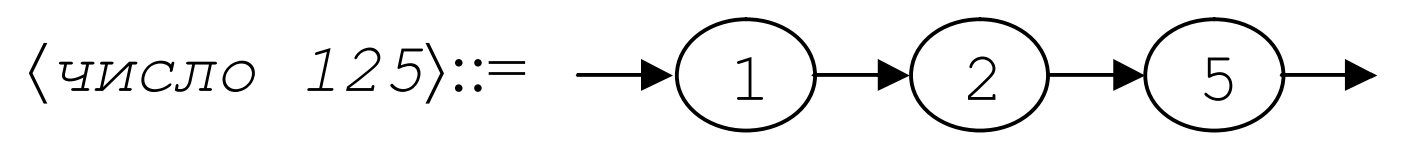
\includegraphics[width=0.65\textwidth]{pics/sdseq.png}  \\~\\     \pause
  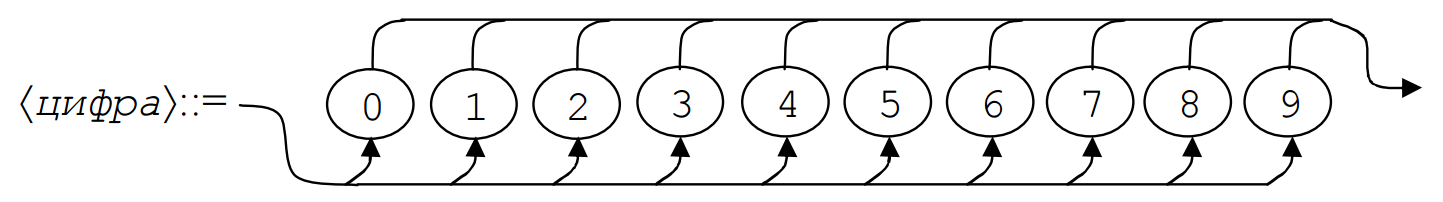
\includegraphics[width=1.0\textwidth]{pics/sddig.png}  \\~\\  \pause   
  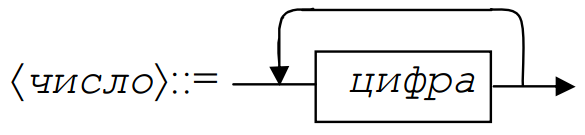
\includegraphics[width=0.45\textwidth]{pics/sdnum.png}  
\end{center}
\end{frame}


\begin{frame}[fragile]
  \transwipe[direction=90]
  \frametitle{Синтаксические диаграммы Вирта}
\begin{center}
  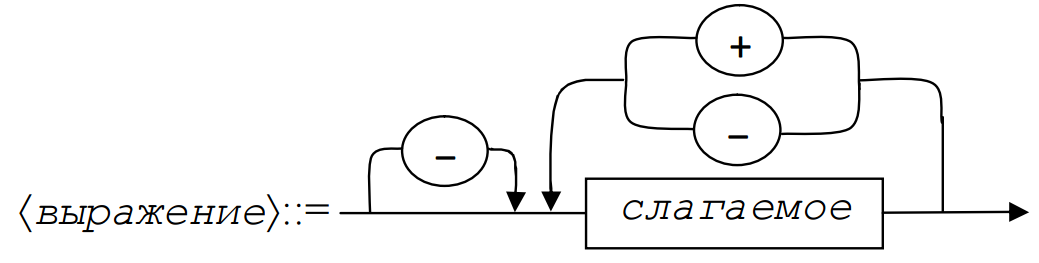
\includegraphics[width=0.75\textwidth]{pics/sdexpr.png}  \\~\\     \pause
  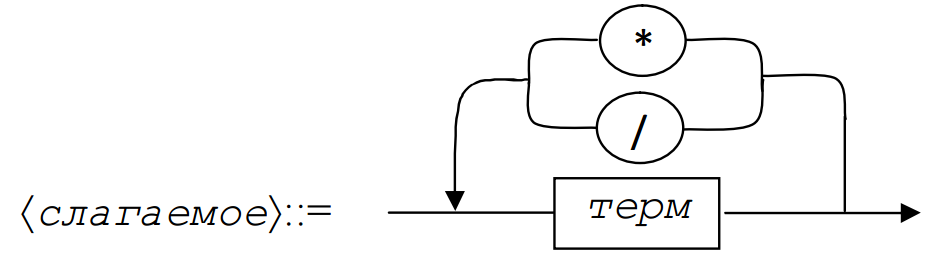
\includegraphics[width=0.75\textwidth]{pics/sdfact.png}  \\~\\  \pause   
  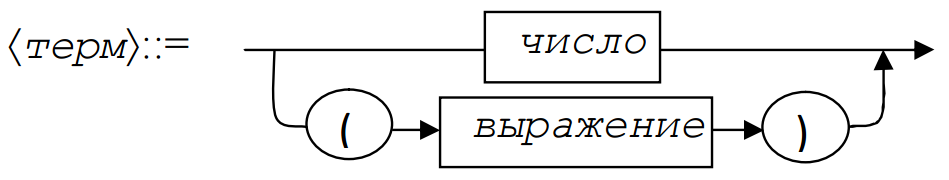
\includegraphics[width=0.75\textwidth]{pics/sdterm.png}  
\end{center}
\end{frame}


\begin{frame}[fragile]
  \transwipe[direction=90]
  \frametitle{Метаязык}
  \begin{itemize}
    \item Язык, на котором дано описание языка
    \begin{itemize}
      \item Естественный язык
      \item Язык металингвистических формул Бэкуса (БНФ)
      \item Синтаксические диаграммы
      \item \textbf{Грамматики}
      \item $\dots$
    \end{itemize}
  \end{itemize}
\end{frame}

\begin{frame}[fragile]
  \transwipe[direction=90]
  \frametitle{Описание языка: формальная грамматика}
  \begin{itemize}
    \item \textbf{Порождающая грамматика $G$} --- это четверка $\langle V_T, V_N, P, S \rangle$

    \begin{itemize}
      \item $V_T$ --- алфавит терминальных  символов (терминалов) 
      \item $V_N$ --- алфавит нетерминальных  символов (нетерминалов)
      \begin{itemize} 
        \item $V_T \cap V_N = \emptyset$ 
        \item $V ::= V_T \cup V_N$
      \end{itemize}
      \item P --- конечное множество правил вида $\alpha \rightarrow \beta$
      \begin{itemize}
        \item $\alpha \in V^* V_N V^*$
        \item $\beta \in V^*$
      \end{itemize}  
      \item S --- начальный нетерминал грамматики,\begin{itemize}
        \item $S  \in N$
      \end{itemize}
    \end{itemize}
  \end{itemize}
\end{frame}

\begin{frame}[fragile]
  \transwipe[direction=90]
  \frametitle{Пример: язык чисел в двоичной системе счисления}

\begin{center}
  $V_T = \{ 0, 1, - \} V_N = \{ S, N, A \}$
\end{center}

\begin{tabular}{p{3cm} | p{4cm} | p{3cm}}

\[
\begin{array}{rcl}
S& \rightarrow & 0 \\
S& \rightarrow & N \\
S& \rightarrow & - N \\
N& \rightarrow & 1 A \\
A& \rightarrow & 0 A \\
A& \rightarrow & 1 A \\
A& \rightarrow & \varepsilon \\
\end{array}
\]

& \pause

\[
\begin{array}{rcl}
S& \rightarrow & 0 \mid N \mid - N  \\
N& \rightarrow & 1 A \\
A& \rightarrow & 0 A \mid 1 A  \mid \varepsilon\\
\end{array}
\]

& \pause

\[
\begin{array}{rcl}
S& \rightarrow & 0 \mid [-] N  \\
N& \rightarrow & 1 A \\
A& \rightarrow & (0 \mid 1) A  \mid \varepsilon\\
\end{array}
\]

\end{tabular}
\end{frame}

\begin{frame}[fragile]
  \transwipe[direction=90]
  \frametitle{Отношение непосредственной выводимости}
  \begin{itemize}
    \item $\alpha \rightarrow \beta \in P$
    \item $\gamma, \delta \in V^*$
    \item $\gamma \alpha \delta \Rightarrow \gamma \beta \delta$: $\gamma \beta \delta$ \textbf{непосредственно выводится} из $\gamma \alpha \delta$ при помощи правила $\alpha \rightarrow \beta$
  \end{itemize}
\end{frame}

\begin{frame}[fragile]
  \transwipe[direction=90]
  \frametitle{Отношение непосредственной выводимости: пример}
  \[
  \begin{array}{rcl}
  S& \rightarrow & 0 \mid N \mid - N  \\
  N& \rightarrow & 1 A \\
  A& \rightarrow & 0 A \mid 1 A  \mid \varepsilon\\
  \end{array}
  \]

\vspace{10pt}

\[S \derives[] -N\]

\[-N \derives[] -1A\]

\[-1A \derives[] -11A\]
\end{frame}


\begin{frame}[fragile]
  \transwipe[direction=90]
  \frametitle{Отношение выводимости}
  
  \begin{center}
    \textbf{Отношение выводимости} является рефлексивно-транзитивным замыканием отношения непосредственной выводимости
  \end{center}

  \begin{itemize}
    \item $\alpha_0, \alpha_1, \alpha_2, \dots, \alpha_n \in V^*$
    \item $\alpha_0 \Rightarrow \alpha_1 \Rightarrow \alpha_2 \Rightarrow \dots \Rightarrow \alpha_n$
    \item $\alpha_0 \derives \alpha_n$: $\alpha_n$ \textbf{выводится} из $\alpha_0$
  \end{itemize}
\end{frame}


\begin{frame}[fragile]
  \transwipe[direction=90]
  \frametitle{Отношение выводимости: пример}
  
  \[
  \begin{array}{rcl}
  S& \rightarrow & 0 \mid N \mid - N  \\
  N& \rightarrow & 1 A \\
  A& \rightarrow & 0 A \mid 1 A  \mid \varepsilon\\
  \end{array}
  \]

  \[ S \Rightarrow - N \Rightarrow - 1 A \Rightarrow - 1 1 A \derives - 1 1 0 1 A \Rightarrow - 1 1 0 1 \]
\end{frame}

\begin{frame}[fragile]
  \transwipe[direction=90]
  \frametitle{Отношение выводимости: свойства}

  \begin{itemize}
    \item Транзитивность: $\forall \alpha, \beta, \gamma \in V^*: \ \alpha \derives \beta, \beta \derives \gamma \text{ следовательно } \alpha \derives \gamma$
    \item Рефлексивность: $\forall \alpha \in V^*: \ \alpha \derives \alpha$
  \end{itemize}

  \begin{itemize}
    \item $\alpha_0 \derives[+] \alpha_n$: вывод использует хотя бы одно правило грамматики
    \item $\alpha_0 \derives[k] \alpha_n$: вывод происходит за $k$ шагов
  \end{itemize}
\end{frame}


\begin{frame}[fragile]
  \transwipe[direction=90]
  \frametitle{Левосторонний вывод}

\begin{center}
  На каждом шагу заменяем самый \textbf{левый} нетерминал
\end{center}

\[
  \begin{array}{rcl}
  S& \rightarrow & A A \mid s  \\
  A& \rightarrow & A A \mid B b \mid a \\
  B& \rightarrow & c \mid d 
  \end{array}
\]

\[ \boldsymbol{S} \derives[] \boldsymbol{A} A \derives[] \boldsymbol{B} b A \derives[] c b \boldsymbol{A} \derives[] c b \boldsymbol{A} A \derives[] c b a \boldsymbol{A} \derives[] c b a a \]

\begin{center}
  Аналогично определяется \textbf{правосторонний} вывод
\end{center}

\end{frame}


\begin{frame}[fragile]
  \transwipe[direction=90]
  \frametitle{Язык, порождаемый грамматикой $G = \langle V_T, V_N, P, S \rangle$}
\[ L(G) = \{ \omega \in V_T^* \mid S \derives \omega \} \]
\end{frame}

\begin{frame}[fragile]
  \transwipe[direction=90]
  \frametitle{Эквивалентность грамматик}
\begin{center}
  Грамматики $G_1$ и $G_2$ \textbf{эквивалентны}, если $L(G_1) = L(G_2)$ 
\end{center}

\pause
  
\begin{tabular}{p{0.5\textwidth} | p{0.5\textwidth}}

\[ 
  \begin{array}{rcl}
  V_T &=& \{ 0, 1, - \} \\
  V_N &=& \{ S, N, A \} \\~\\
  S& \rightarrow & 0 \mid N \mid - N  \\
  N& \rightarrow & 1 A \\
  A& \rightarrow & 0 A \mid 1 A  \mid \varepsilon\\
  \end{array}
\]          
  
&

\[
  \begin{array}{rcl}
  V_T &=& \{ 0, 1, - \} \\
  V_N &=& \{ S, A \} \\~\\
  S& \rightarrow & 0 \mid 1 A  \mid - 1 A  \\
  A& \rightarrow &  0 A \mid 1 A  \mid \varepsilon\\
  \end{array}
\]    
\end{tabular} 

\end{frame}

\begin{frame}[fragile]
  \transwipe[direction=90]
  \frametitle{Контекстно-свободная грамматика}
    \begin{center}
      \textbf{Контекстно-свободная грамматика} --- грамматика, все правила которой имеют вид $A \rightarrow \alpha, A \in V_N, \alpha \in V^*$
    \end{center}
\end{frame}

\begin{frame}[fragile]
  \transwipe[direction=90]
  \frametitle{Дерево вывода}
  
  Дерево является \textbf{деревом вывода} для $G = \langle V_N, V_T, P, S\rangle$, если:  
  \begin{itemize}
    \item Каждый узел помечен символом из алфавита $V$
    \item Метка корня --- $S$
    \item Листья помечены терминалами, остальные узлы --- нетерминалами
    \item Если узлы $n_0, \dots, n_k$ --- прямые потомки узла $n$, перечисленные слева направо, с метками $A_0, \dots, A_k$; метка $n$ --- $A$, то $A \rightarrow A_0 \dots A_k \in P$
  \end{itemize}
\end{frame}

\begin{frame}[fragile]
  \transwipe[direction=90]
  \frametitle{Пример дерева вывода}
\begin{center}

\[ G = \langle \{ S, A \}, \{ a, b \}, \{ S \rightarrow a A S \mid a, A \rightarrow S b A \mid b a \mid SS \}, S\rangle \]

\[ S \Rightarrow aAS \Rightarrow a S b A S \Rightarrow a a b A S \Rightarrow a a b b a S \Rightarrow a a b b a a \]
    
\begin{forest}
  [S
    [a]
    [A
      [S
        [a]
      ]
      [b]
      [A
        [b]
        [a]
      ]
    ]
    [S
      [a]
    ]
  ]
\end{forest}
\end{center}
\end{frame}

\begin{frame}[fragile]
  \transwipe[direction=90]
  \frametitle{Вывод и дерево вывода}
  \begin{rutheorem}[]
    Пусть $G = \langle V_N, V_T, P, S \rangle$ --- КС-грамматика
    
    Вывод $S \derives \alpha$, где $\alpha \in V^*, \alpha \neq \varepsilon$ существует $\Leftrightarrow$ существует дерево вывода в грамматике G с результатом $\alpha$
  \end{rutheorem}

\begin{center}
  Упражнение: доказать теорему
\end{center}
\end{frame}

\end{document}
